\documentclass{beamer}
\usetheme{Boadilla}
\usecolortheme{orchid}

\usepackage[T1]{fontenc}
\usepackage[utf8]{inputenc}
\usepackage[french]{babel}
\usepackage{stackengine}

\addtobeamertemplate{navigation symbols}{}{%
    \usebeamerfont{footline}%
    \usebeamercolor[fg]{footline}%
    \hspace{1em}%
    \insertframenumber/\inserttotalframenumber
}
\usepackage{ulem}
\usepackage{tkz-tab}
\setbeamertemplate{blocks}[rounded]%
[shadow=true]
\AtBeginSection{%
    \begin{frame}
        \tableofcontents[sections=\value{section}]
    \end{frame}
}

\newenvironment*{remerciements}{%
  \renewcommand*{\abstractname}{Remerciements}
  \begin{abstract}
}{
  \end{abstract}
}

\title[Swap Cross-Blockchain]{Echange de jetons inter-blockchains}
\subtitle{Projet de fin d'études: Master 2 Informatique Option Fiabilité et sécurité informatique 2022-2023}
\author[M2 FSI]{VOLPE Dorian, ROTONDO Eloïse, TESTUD Romain,\\DE CAMPOU Louis, JOLY Amaury  \\ \textbf{Encadrants :} TRAVERS Corentin, LABOUREL Arnaud \\[2ex] 
\includegraphics[scale=0.1]{./img/amu.png}}
\institute[Aix-Marseille Université]{M2 Fiabilité et sécurité informatique}
\date{\today}

\begin{document}

\maketitle

\begin{frame}
  \begin{remerciements}
    Merci à M. TRAVERS Corentin et M. LABOUREL Arnaud pour la proposition de ce sujet et son encadrement.
  \end{remerciements}
  \begin{abstract}
    abstract
  \end{abstract}
\end{frame}

\begin{frame}{Table des matières}
  \tableofcontents
\end{frame}

\section{Introduction}
\begin{frame}{Centralisé}
    \begin{block}{Le centralisé offre\dots}
        \begin{itemize}
            \item Diversité d'acteurs.
            \item Accessibilité.
            \item Multiples fonctionnalités.
        \end{itemize}
    \end{block}
    \pause
    \begin{block}{Mais\dots}
        \begin{itemize}
            \item Opacité des protocoles.
            \item Failles de sécurité.
            \item Collecte des données.
        \end{itemize}
    \end{block}
\end{frame}


\begin{frame}{Décentralisé}
    \begin{block}{Le décentralisé offre\dots\dots}
        \begin{itemize}
            \item Pas de tiers de confiance.
            \item Transparence.
            \item Fiabilité accrue.
        \end{itemize}
    \end{block}
    \pause
    \begin{block}{Mais\dots}
        \begin{itemize}
            \item Difficiles d'accès.
            \item Intérêt économique faible.
        \end{itemize}
    \end{block}
\end{frame}

\begin{frame}{Conclusion générale}
    \begin{itemize}
        \item Flou entre centralisé/décentralisé.
        \item Définition variable.
    \end{itemize}
\end{frame}

\begin{frame}
    \begin{figure}
        \begin{figure}
            \centering
            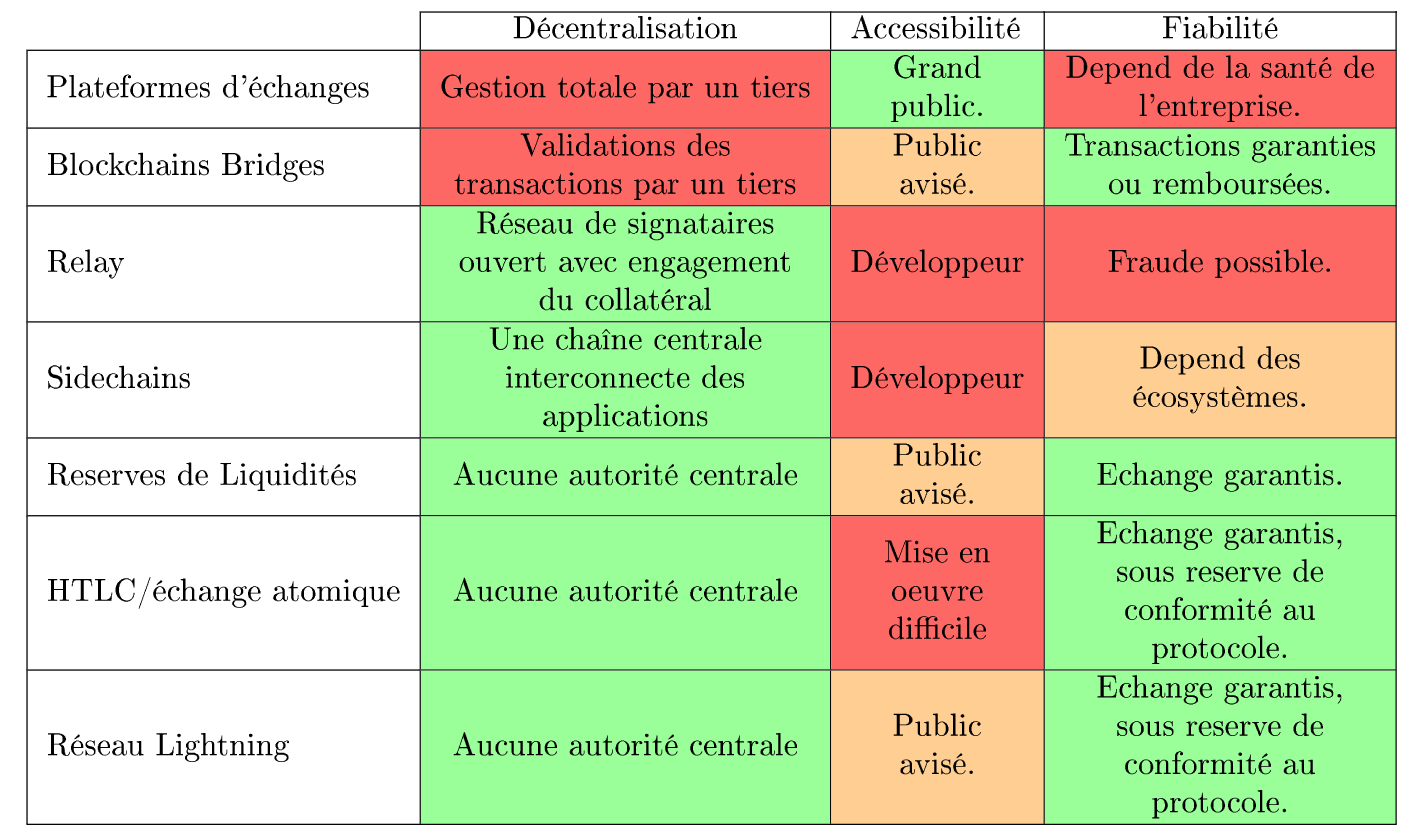
\includegraphics[scale = 0.2]{conclusion/tableau.png}
            \label{fig:recap}
            \caption{Tableau récapitulatif}
        \end{figure}
    \end{figure}
    
\end{frame}
\section{Centralisation}
\begin{frame}{Centralisé}
    \begin{block}{Le centralisé offre\dots}
        \begin{itemize}
            \item Diversité d'acteurs.
            \item Accessibilité.
            \item Multiples fonctionnalités.
        \end{itemize}
    \end{block}
    \pause
    \begin{block}{Mais\dots}
        \begin{itemize}
            \item Opacité des protocoles.
            \item Failles de sécurité.
            \item Collecte des données.
        \end{itemize}
    \end{block}
\end{frame}


\begin{frame}{Décentralisé}
    \begin{block}{Le décentralisé offre\dots\dots}
        \begin{itemize}
            \item Pas de tiers de confiance.
            \item Transparence.
            \item Fiabilité accrue.
        \end{itemize}
    \end{block}
    \pause
    \begin{block}{Mais\dots}
        \begin{itemize}
            \item Difficiles d'accès.
            \item Intérêt économique faible.
        \end{itemize}
    \end{block}
\end{frame}

\begin{frame}{Conclusion générale}
    \begin{itemize}
        \item Flou entre centralisé/décentralisé.
        \item Définition variable.
    \end{itemize}
\end{frame}

\begin{frame}
    \begin{figure}
        \begin{figure}
            \centering
            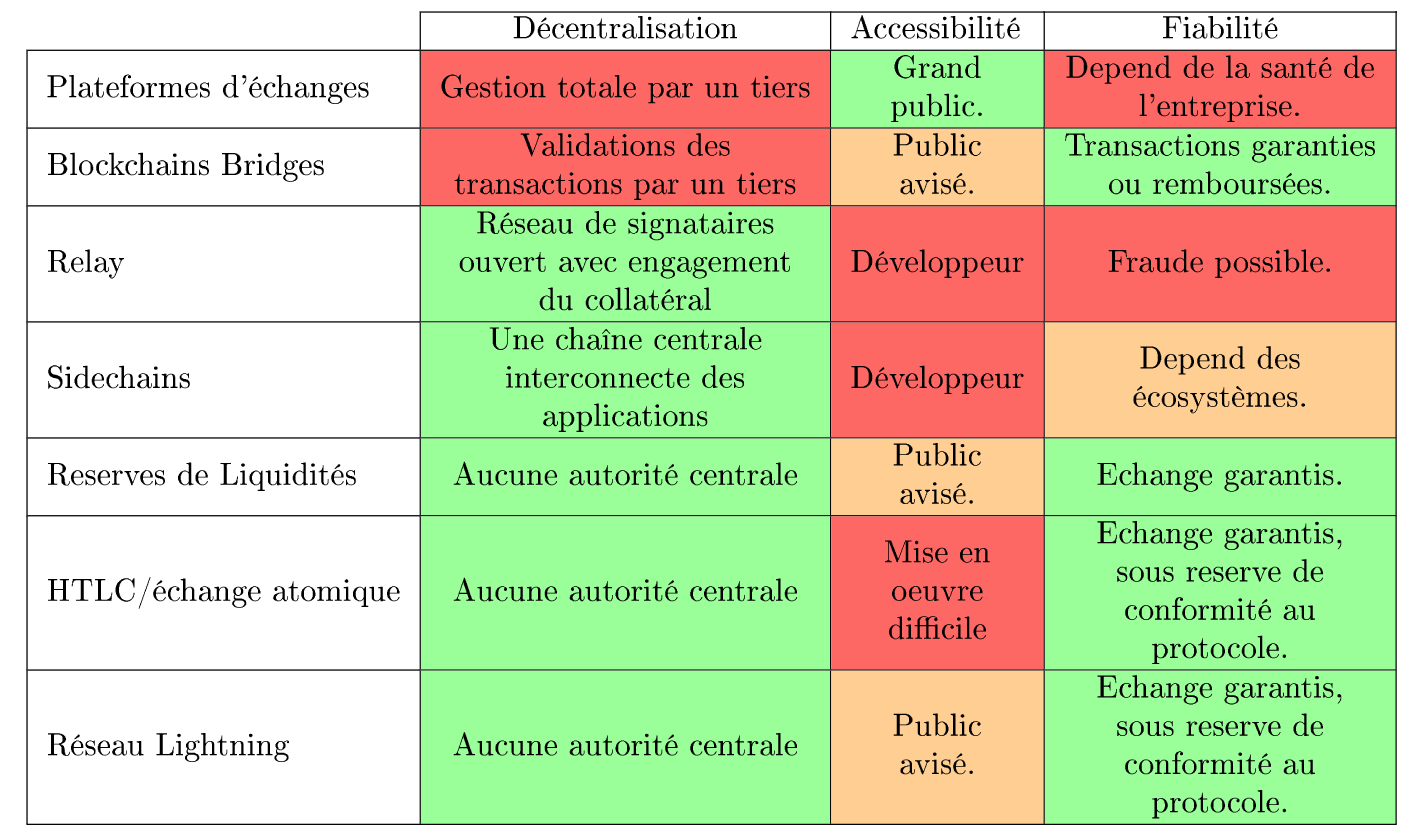
\includegraphics[scale = 0.2]{conclusion/tableau.png}
            \label{fig:recap}
            \caption{Tableau récapitulatif}
        \end{figure}
    \end{figure}
    
\end{frame}
\section{Décentralisation}
\begin{frame}{Centralisé}
    \begin{block}{Le centralisé offre\dots}
        \begin{itemize}
            \item Diversité d'acteurs.
            \item Accessibilité.
            \item Multiples fonctionnalités.
        \end{itemize}
    \end{block}
    \pause
    \begin{block}{Mais\dots}
        \begin{itemize}
            \item Opacité des protocoles.
            \item Failles de sécurité.
            \item Collecte des données.
        \end{itemize}
    \end{block}
\end{frame}


\begin{frame}{Décentralisé}
    \begin{block}{Le décentralisé offre\dots\dots}
        \begin{itemize}
            \item Pas de tiers de confiance.
            \item Transparence.
            \item Fiabilité accrue.
        \end{itemize}
    \end{block}
    \pause
    \begin{block}{Mais\dots}
        \begin{itemize}
            \item Difficiles d'accès.
            \item Intérêt économique faible.
        \end{itemize}
    \end{block}
\end{frame}

\begin{frame}{Conclusion générale}
    \begin{itemize}
        \item Flou entre centralisé/décentralisé.
        \item Définition variable.
    \end{itemize}
\end{frame}

\begin{frame}
    \begin{figure}
        \begin{figure}
            \centering
            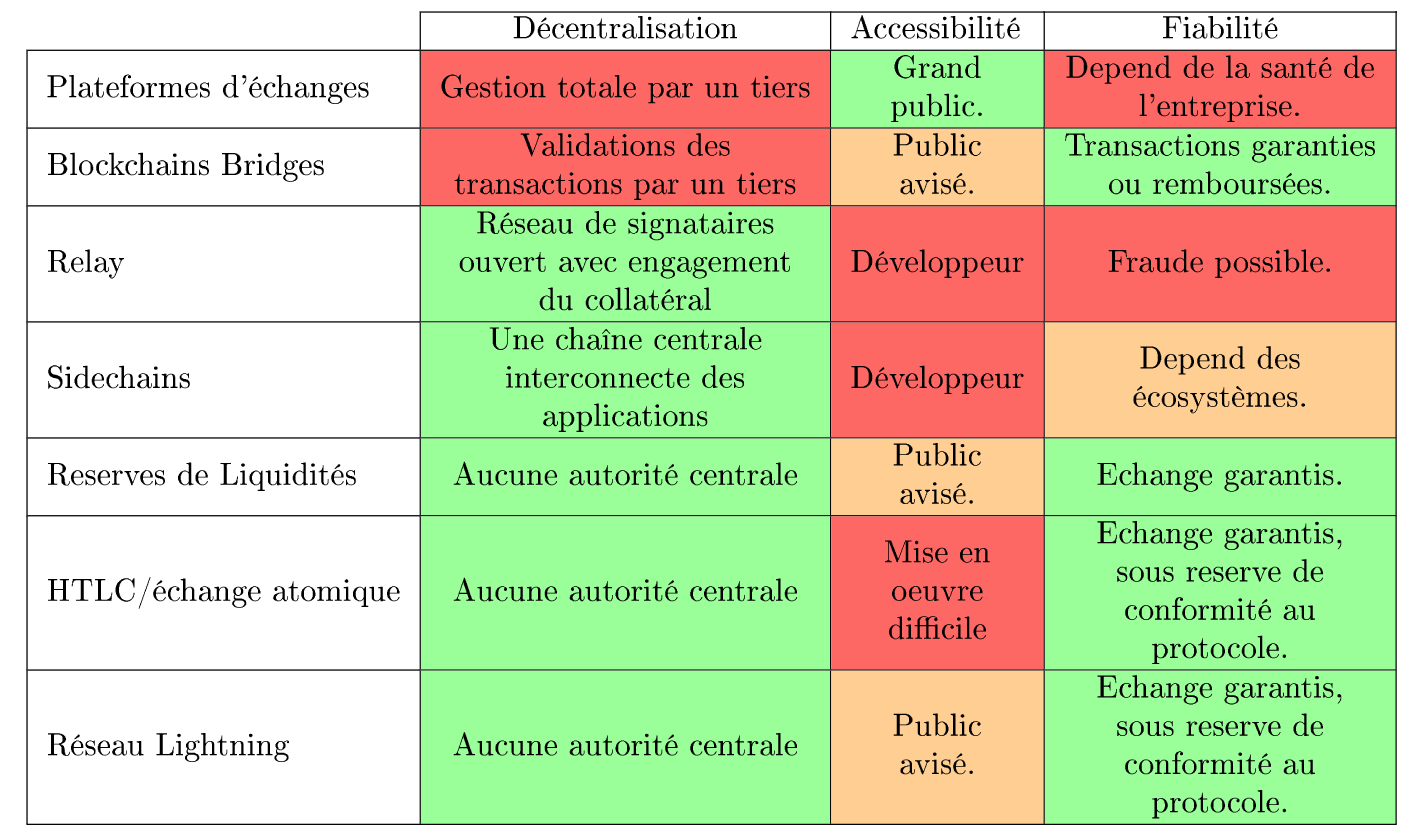
\includegraphics[scale = 0.2]{conclusion/tableau.png}
            \label{fig:recap}
            \caption{Tableau récapitulatif}
        \end{figure}
    \end{figure}
    
\end{frame}
\section{Conclusion}
\begin{frame}{Centralisé}
    \begin{block}{Le centralisé offre\dots}
        \begin{itemize}
            \item Diversité d'acteurs.
            \item Accessibilité.
            \item Multiples fonctionnalités.
        \end{itemize}
    \end{block}
    \pause
    \begin{block}{Mais\dots}
        \begin{itemize}
            \item Opacité des protocoles.
            \item Failles de sécurité.
            \item Collecte des données.
        \end{itemize}
    \end{block}
\end{frame}


\begin{frame}{Décentralisé}
    \begin{block}{Le décentralisé offre\dots\dots}
        \begin{itemize}
            \item Pas de tiers de confiance.
            \item Transparence.
            \item Fiabilité accrue.
        \end{itemize}
    \end{block}
    \pause
    \begin{block}{Mais\dots}
        \begin{itemize}
            \item Difficiles d'accès.
            \item Intérêt économique faible.
        \end{itemize}
    \end{block}
\end{frame}

\begin{frame}{Conclusion générale}
    \begin{itemize}
        \item Flou entre centralisé/décentralisé.
        \item Définition variable.
    \end{itemize}
\end{frame}

\begin{frame}
    \begin{figure}
        \begin{figure}
            \centering
            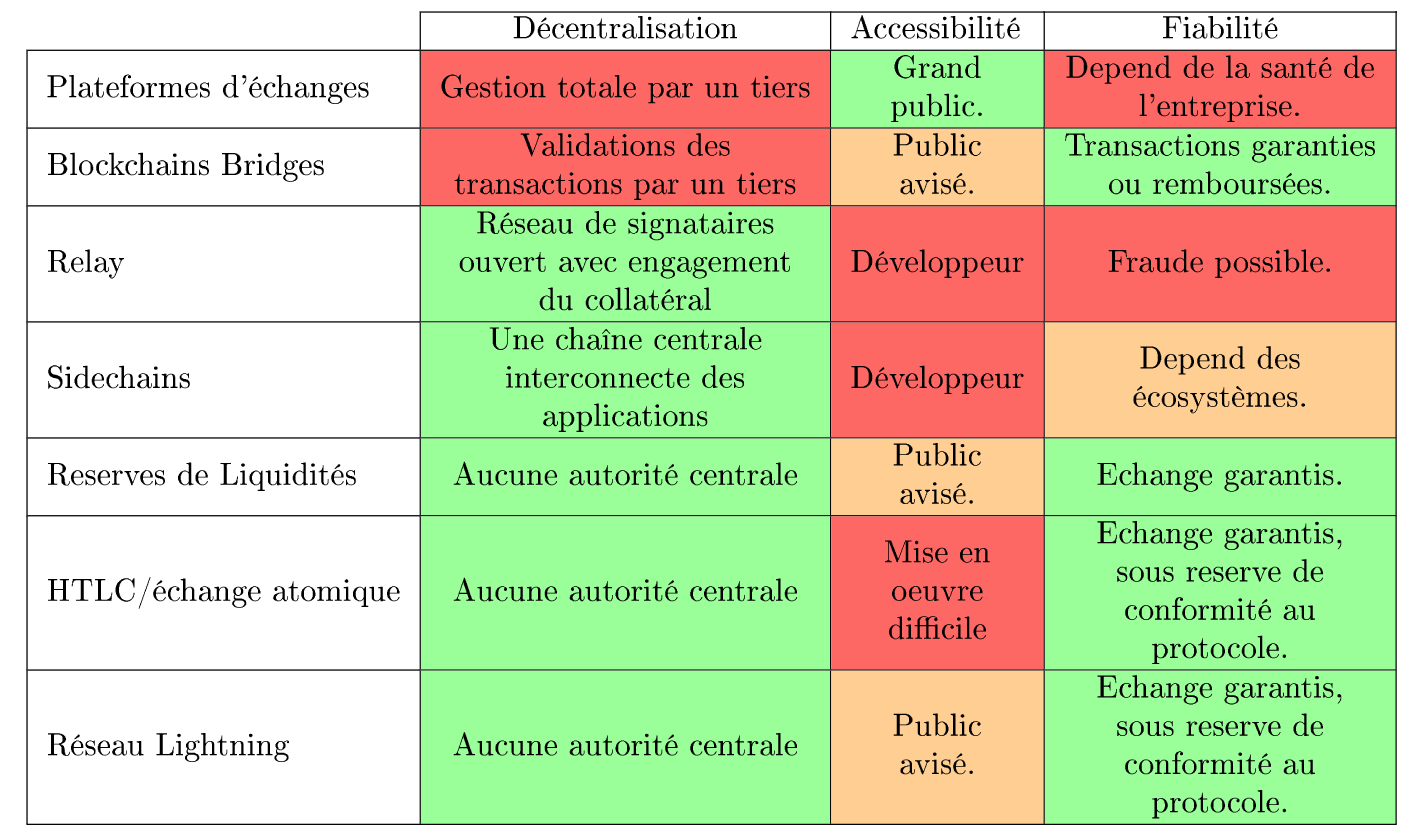
\includegraphics[scale = 0.2]{conclusion/tableau.png}
            \label{fig:recap}
            \caption{Tableau récapitulatif}
        \end{figure}
    \end{figure}
    
\end{frame}

\end{document}